\chapter{Gateway}
A gateway is a device that forwards messages from another device, the client, to a second device, the server or another gateway.
In the following figures, there are two examples of gateways: Layer-3 gateways (routers) and Layer-7 gateways (proxy).
\begin{figure}[h]
\centering
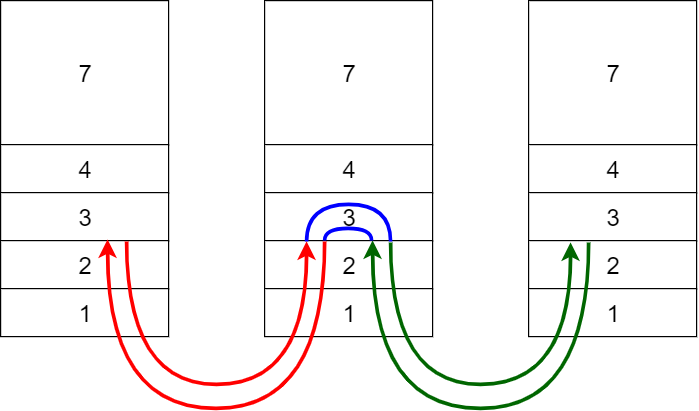
\includegraphics[scale=0.4]{Images/Gateway/gateway_3}
\caption{\footnotesize{Router (Layer-3 gateway).}}\label{gateway_3}
\end{figure}
\begin{figure}[h]
\centering
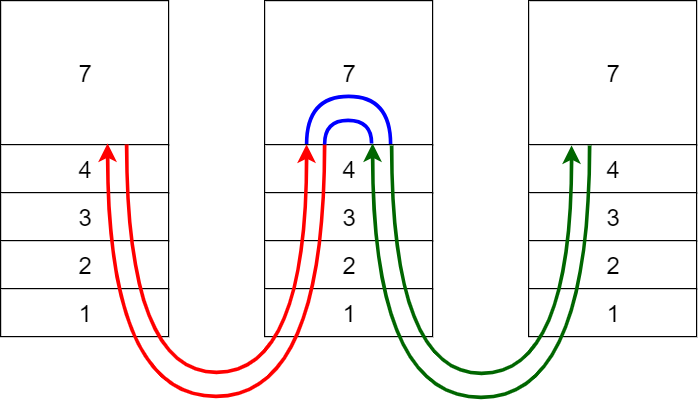
\includegraphics[scale=0.4]{Images/Gateway/gateway_7}
\caption{\footnotesize{Proxy (Layer-7 gateway).}}\label{gateway_7}
\end{figure}

\section{Proxy}
A Layer-7 gateway is also called proxy. It works as an intermediary between two identical protocols (Figure \ref{proxy}). Instead of Layer-3 gateways, proxy can also see the full stream of data, analyze HTTP headers and implement new functions. 
\begin{figure}[h]
\centering
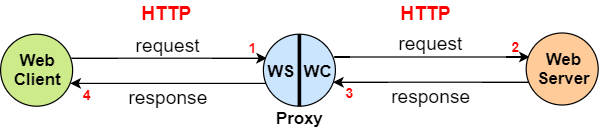
\includegraphics[scale=0.42]{Images/Gateway/proxy}
\caption{\footnotesize{Example of proxy use.}}\label{proxy}
\end{figure}
The main possible functions are:
\begin{itemize}
\item{\textbf{Caching}\\
It's used to reduce traffic directed to the server. The proxy does the most expensive job, managing all the requests of the same page of the server. \\
After the request of the page for the first time, the proxy asks the page to the server and then stores in its system, before replying. Hence the next clients requests of the same page will be manage only by proxy because the page was already stored in its system.\\
In this case the server needs to manage only a request by proxy and provide a response to proxy.
\begin{figure}[h]
\centering
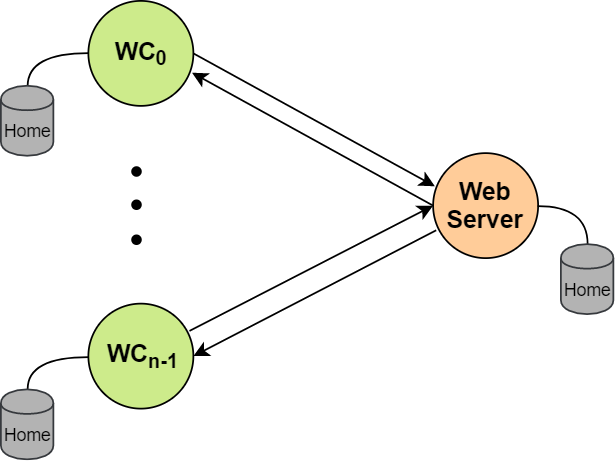
\includegraphics[scale=0.38]{Images/Gateway/proxy_cache_no}
\caption{\footnotesize{Example of caching without proxy.}}\label{proxy_cache_no}
\end{figure}
\begin{figure}[h]
\centering
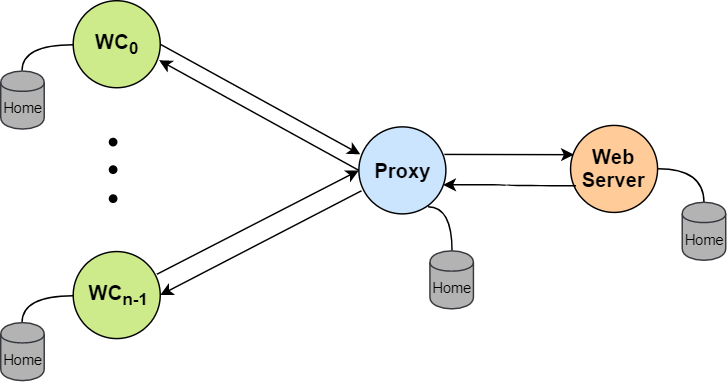
\includegraphics[scale=0.4]{Images/Gateway/proxy_cache}
\caption{\footnotesize{Example of caching using proxy.}}\label{proxy_cache}
\end{figure}
}
\item{\textbf{Filtering}\\
The proxy can do two actions:
\begin{itemize}
\item{\textbf{Filtering the requested resource by the client}\\
there are many companies that doesn't give access to some services (E.g. no access to Facebook, Youtube, ...).\\
We cannot use a filtering approach at lower levels because in some cases clients can access to services through intermediate addresses, different from the one we want to reach. Hence we need to analyze the HTTP request at upper layer.}
\item{\textbf{Filtering the content of the response}\\
for parent control approach.}
\end{itemize}
\begin{figure}[h]
\centering
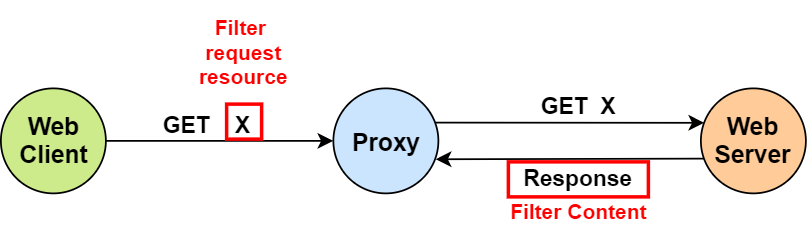
\includegraphics[scale=0.4]{Images/Gateway/proxy_filter}
\caption{\footnotesize{Example of proxy filtering.}}\label{proxy_filter}
\end{figure}
}
\item{\textbf{Web Application Firewall (WAF)}\\
The proxy is specialized and used to block suspicious requests. This is done by analyzing request content, looking for not secure pattern.\\
A possible pattern can be \textit{".."} in the path of the resource, that could give access to not accessible part of the File System (injection). Another possible pattern could be a suspicious parameter for a web application to manage SQL database (SQL injection).
\begin{figure}[h]
\centering
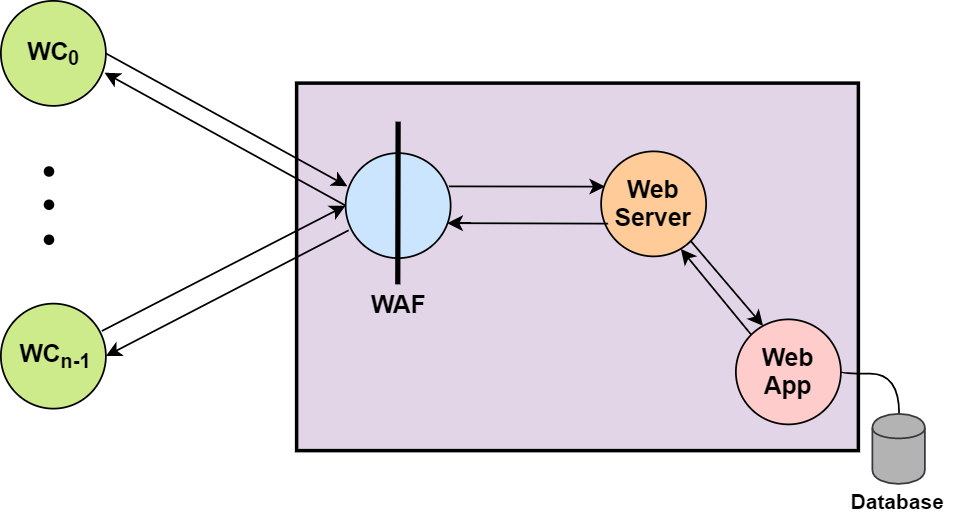
\includegraphics[scale=0.4]{Images/Gateway/proxy_waf}
\caption{\footnotesize{Example of WAF use.}}\label{proxy_waf}
\end{figure}
}
\item{\textbf{Load Balancing}\\
The proxy is a load balancer for the clients requests to the server.\\
There are many servers to manage requests by client. The client makes the request of the web page but in the reality it's talking with the proxy, that manage the request by sending it to a particular server.\\
This action is repeated for each client's request. Hence the client thinks that is talking to one server but in reality, the proxy distribute the requests among several servers. 
\begin{figure}[h]
\centering
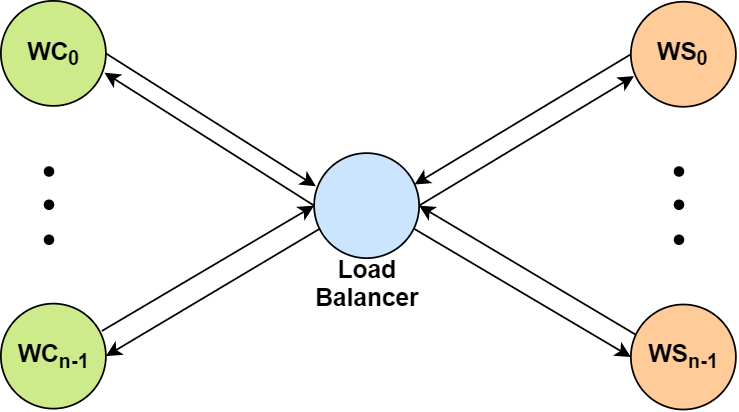
\includegraphics[scale=0.4]{Images/Gateway/proxy_load}
\caption{\footnotesize{Example of load balancing through proxy.}}\label{proxy_load}
\end{figure}
}
\end{itemize}

\subsection{Proxy implementation}
If the client wants to use a proxy, he needs to modify its behaviour, following the following steps:
\begin{enumerate}
\item{\textbf{Connection of Client to Web Proxy instead of the server}\\
The client needs to change address and port w.r.t. proxy ones, instead of server ones.}
\item{\textbf{Specify the absolute path of the requested resource}\\
Otherwise proxy doesn't to which one the message needs to be sent. Hence he couldn't forward as it is the request.
}
\end{enumerate}